% =====================================================================
% Guía del estudiante -- Geometría 9° -- Trimestre I
% María Mercedes Cantillo · Colegio San Alberto Magno
% ---------------------------------------------------------------------
% Plan: guia-periodo-I-semejanza-medicion.plan.md (y curriculo/plan-anual.md).
% Cada \tema tiene \label{tema:...} para que las clases lo citen con
% \refguia{tema:...}. No borrar el .aux de esta guía.
%
% Compilar:  latexmk -pdf guia-periodo-I-semejanza-medicion.tex
% =====================================================================
% Plan del trimestre aprobado por la docente el 2026-09-18. Esta guía es todavía el borrador de
% la generación rápida del 2026-09-14: falta rehacerla con el proceso de tres etapas.
\documentclass[11pt]{article}
\makeatletter\def\input@path{{../../../../plantillas/estilo/}}\makeatother
\usepackage{mmcantillo}

% ======================== DATOS DE LA GUÍA ============================
\tipodocumento{Guía del estudiante}
\asignatura{Geometría}
\titulo{Medir lo inalcanzable: semejanza, Thales y Pitágoras}
\grado{9°}
\periodo{I}
\hiloconductor{Eratóstenes mide la Tierra con una sombra}
% ======================================================================
% DBA: matematicas grado 9 · DBA 5 — Utiliza teoremas, propiedades y relaciones
%      geométricas (teorema de Thales y el teorema de Pitágoras) para proponer y
%      justificar estrategias de medición y cálculo de longitudes.
%      DBA 6 — Conjetura acerca de las regularidades de las formas bidimensionales
%      y tridimensionales y realiza inferencias a partir de los criterios de
%      semejanza, congruencia y teoremas básicos.

\begin{document}

\encabezado

% ---------------------------------------------------------------------
% 1. Frase introductoria
% ---------------------------------------------------------------------
% verificado: https://portalegalileo.museogalileo.it/egjr.asp?c=36261 — Il Saggiatore (Roma, 1623): «Egli è scritto in lingua matematica, e i caratteri son triangoli, cerchi, ed altre figure geometriche»
\frase{La filosofía está escrita en este grandísimo libro que tenemos siempre
abierto ante los ojos (quiero decir, el universo), pero no se puede entender si
antes no se aprende su lengua y se conocen los caracteres en que está escrito.
Está escrito en lengua matemática, y sus caracteres son triángulos, círculos y
otras figuras geométricas.}
{Galileo Galilei, \emph{El ensayador} (1623), trad. propia~\cite{galileo1623}}

% ---------------------------------------------------------------------
% 2. Introducción
% ---------------------------------------------------------------------
\seccion{Introducción}

¿Cómo se mide la altura de un árbol sin subirse a él, el ancho de un lago sin
cruzarlo o el tamaño de la Tierra sin darle la vuelta? Con triángulos. En este
trimestre aprenderemos a reconocer cuándo dos figuras tienen la misma forma
(\textbf{semejanza}) o la misma forma y el mismo tamaño (\textbf{congruencia}), y a
usar dos teoremas clásicos, el de \textbf{Thales} y el de \textbf{Pitágoras}, para
medir lo que no se puede alcanzar con una cinta métrica. También aprenderemos a
preguntarnos qué tan confiable es una medida.

Nuestro hilo conductor es uno de los experimentos más famosos de la historia. Hace
unos 2\,250 años, en Alejandría (Egipto), el bibliotecario Eratóstenes calculó el
tamaño de toda la Tierra con la sombra de un palo, un ángulo y una distancia entre
dos ciudades. Cada tema de esta guía es un paso de su razonamiento, y al final
podrás repetir su experimento en el colegio.

\textbf{Al terminar este trimestre podrás:}
\begin{itemize}
  \item decidir si dos triángulos son semejantes o congruentes y justificarlo con un criterio;
  \item usar el teorema de Thales para calcular longitudes con rectas paralelas y sombras;
  \item usar el teorema de Pitágoras para medir distancias de forma indirecta;
  \item proponer una estrategia de medición, justificarla y decir qué tan precisa es.
\end{itemize}

Este trimestre trabaja dos Derechos Básicos de Aprendizaje del Ministerio de
Educación Nacional~\cite{mendba}:

\begin{dba}[Grado 9 · DBA 5]
Utiliza teoremas, propiedades y relaciones geométricas (teorema de Thales y el
teorema de Pitágoras) para proponer y justificar estrategias de medición y cálculo
de longitudes.
\end{dba}

\begin{dba}[Grado 9 · DBA 6]
Conjetura acerca de las regularidades de las formas bidimensionales y
tridimensionales y realiza inferencias a partir de los criterios de semejanza,
congruencia y teoremas básicos.
\end{dba}

% ---------------------------------------------------------------------
% 3. Marco teórico
% ---------------------------------------------------------------------
\seccion{Marco teórico}

\subsubsection*{Eratóstenes, el bibliotecario llamado «Beta»}

Eratóstenes nació en Cirene (en la actual Libia) hacia el 276 a.\,C. y murió hacia
el 194 a.\,C. Hacia el 240 a.\,C. se convirtió en el tercer bibliotecario de la
Biblioteca de Alejandría, el mayor centro de estudio del mundo griego. Escribió de
geografía, astronomía, matemáticas y poesía. Sus contemporáneos lo apodaban
«Beta», la segunda letra del alfabeto griego: sobresalía en muchos campos, aunque
según ellos no llegaba al primer puesto en ninguno~\cite{mactutoreratostenes}.

\subsubsection*{Una sombra, un ángulo y una distancia}

La versión más conocida de su medición la cuenta Cleomedes, un maestro de
astronomía de la época romana, en su libro \emph{El cielo}~\cite{cleomedes}. En
Siena (la actual Asuán), al mediodía del solsticio de verano, el Sol estaba justo
encima: los gnomones (palos verticales usados como relojes de sol) no daban
sombra. A la misma hora, en Alejandría, más al norte, la sombra de un gnomon
formaba con la vertical un ángulo de $\frac{1}{50}$ de circunferencia, es decir,
$\num{7,2}^\circ$. Eratóstenes supuso que el Sol está tan lejos que sus rayos llegan
paralelos a la Tierra. Entonces, por los ángulos entre paralelas, el arco entre las
dos ciudades también es $\frac{1}{50}$ de la circunferencia de la Tierra. Como entre
Siena y Alejandría había unos 5\,000 estadios, la circunferencia completa mediría
$50 \cdot 5\,000 = 250\,000$ estadios~\cite{cleomedes, mactutoreratostenes}.

¿Cuánto es eso en kilómetros? Nadie lo sabe con certeza, porque el
\emph{estadio} no era una unidad única: los historiadores proponen valores entre
unos 157 y unos 185 metros, y según el que se escoja el resultado de Eratóstenes
queda muy cerca del valor real (unos $40\,000$~km) o se pasa en más de un
10~\%~\cite{mactutoreratostenes}. Su método era correcto; la precisión dependía de
sus instrumentos y de sus unidades. Esa es la segunda lección del trimestre.

\subsubsection*{Dos teoremas para medir}

El razonamiento de Eratóstenes usa la geometría que los griegos habían reunido:
rectas paralelas cortadas por secantes y triángulos de la misma forma, que en
nuestro idioma asociamos con el nombre de Thales de Mileto, y el teorema de
Pitágoras, que relaciona los lados de un triángulo rectángulo. Del teorema de
Pitágoras se conocen cientos de demostraciones. Una de las más cortas la publicó
en 1876 un congresista de los Estados Unidos, James A. Garfield, que años después
sería presidente de su país: calculó el área de un trapecio de dos maneras
distintas~\cite{garfield}.

\subsubsection*{Henrietta Leavitt: medir lo que está aún más lejos}

Veintidós siglos después de Eratóstenes, la pregunta era otra: ¿a qué distancia
están las estrellas? En el Observatorio del Harvard College, \textbf{Henrietta Swan
Leavitt} estudiaba en placas fotográficas las estrellas variables, que cambian de
brillo en ciclos regulares. En 1912 publicó que, en 25 de esas estrellas de la
Nube Menor de Magallanes, las más brillantes tardaban más en completar su ciclo:
bastaba medir el periodo para conocer el brillo real, y al compararlo con el brillo
que se ve desde la Tierra, calcular la distancia~\cite{leavitt}. Con esa
relación, que hoy lleva su nombre, se midieron después las distancias a otras
galaxias. Como Eratóstenes, midió lo inalcanzable con una estrategia indirecta.

Los criterios y ejemplos de los temas siguen el módulo de Geometría de las Guías de
Apoyo~\cite{quintero}; las preguntas del Icfes se reproducen textualmente del
cuadernillo oficial~\cite{icfes2026}.

% ---------------------------------------------------------------------
% 4. Temas
% ---------------------------------------------------------------------
\tema{Semejanza de figuras}\label{tema:semejanza}

\begin{hilo}
En la Biblioteca de Alejandría, Eratóstenes dibuja mapas del mundo conocido. Un
mapa es una figura \emph{semejante} al terreno: la misma forma, otro tamaño. Esa
idea ---misma forma, distinto tamaño--- es la que usará para medir la Tierra.
\end{hilo}

\begin{definicion}[Figuras semejantes]
Dos figuras son \textbf{semejantes} si tienen los mismos ángulos, uno a uno, y sus
lados correspondientes son proporcionales. El cociente entre lados
correspondientes es la \textbf{razón de semejanza} $k$. Se escribe
$\triangle ABC \sim \triangle A'B'C'$.
\end{definicion}

\begin{teorema}[Criterios de semejanza de triángulos]
Dos triángulos son semejantes si cumplen alguno de estos criterios:
\begin{enumerate}[label=\textbf{\arabic*.}]
  \item \textbf{AA:} dos ángulos de uno son iguales a dos ángulos del otro (el
        tercero también lo es, porque los tres suman $180^\circ$).
  \item \textbf{LAL:} dos lados son proporcionales y el ángulo comprendido entre
        ellos es igual.
  \item \textbf{LLL:} los tres lados son proporcionales.
\end{enumerate}
\end{teorema}

% Ejemplo del recurso: módulo de Geometría, Tema 2, Semejanza, Ejemplo 3 (15/5 = 9/3 = 12/4 = 3)
\begin{ejemplo}[Criterio LLL]
Los triángulos de lados $5$, $3$, $4$ y $15$, $9$, $12$ son semejantes, porque
$\frac{15}{5} = \frac{9}{3} = \frac{12}{4} = 3$. La razón de semejanza es $k = 3$.
Ojo: si los lados se multiplican por $3$, el área se multiplica por $3^2 = 9$
(el primero es rectángulo, de área $6$, y el segundo tiene área $54$).
\end{ejemplo}

\begin{aplicacion}[Planos y maquetas]
Los planos de una casa se dibujan a escala, por ejemplo $1:100$: cada centímetro
del plano representa un metro. El plano y la casa son figuras semejantes, así que
los ángulos se conservan y todas las longitudes se dividen por el mismo número. Así
un arquitecto puede calcular longitudes reales midiendo sobre el papel.
\end{aplicacion}

\begin{preguntas}
% Ejercicio: semejanza-escala-5-003
\pregunta Rectángulo A: 5 cm de longitud y 19 cm de ancho; rectángulo B: 20 cm y
38 cm; rectángulo C: 15 cm y 57 cm. ¿Qué rectángulos son figuras semejantes?
Explica por qué.
\espacio{2.5cm}
% Ejercicio: icfes-cuadernillo-2026-007
\Needspace{16\baselineskip}
\pregunta (Icfes, Saber 11.º, 2026, pregunta 7.) La figura muestra el portalápices de Eliécer. Él sabe que es posible colocar un
caucho de 18 cm de perímetro alrededor de la base sin estirarlo, pero a medida
que sube el caucho por el portalápices, este se estira hasta que, en la boca del
portalápices, su perímetro es 24 cm.

\begin{center}
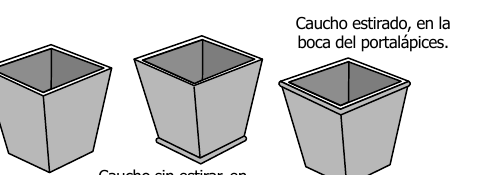
\includegraphics[width=0.55\linewidth]{figuras/icfes-2026-p7.png}
\end{center}

El portalápices tiene base y boca cuadrada, por lo cual Eliécer afirma: «Como los
perímetros de la base y la boca del portalápices están en relación
$\frac{18}{24} = \frac{3}{4}$, el área de la base debe ser también tres cuartas
partes del área de la boca del portalápices». ¿Es verdadera esta afirmación?
\begin{opciones}
  \item No, porque la medición se realiza con el mismo caucho y, por tanto, las
        áreas de la base y la boca deben ser iguales.
  \item Sí, porque el caucho se estira dependiendo del área que encierre, por lo que
        las relaciones de las áreas y los perímetros son iguales.
  \item No, porque la relación obtenida se cumple para las longitudes de los lados,
        pero al calcular las áreas, la razón obtenida se eleva al cuadrado.
  \item Sí, porque como las figuras son semejantes, todas sus medidas deben tener la
        misma razón que los perímetros.
\end{opciones}
Justifica tu elección con los lados de los dos cuadrados.
\espacio{2.5cm}
\end{preguntas}

\begin{resumen}
\begin{itemize}
  \item Semejantes: mismos ángulos y lados proporcionales, con razón $k$.
  \item Criterios para triángulos: AA, LAL y LLL.
  \item Si las longitudes se multiplican por $k$, las áreas se multiplican por $k^2$.
\end{itemize}
\end{resumen}

% ---------------------------------------------------------------------
\tema{Congruencia}\label{tema:congruencia}

\begin{hilo}
Para conocer la distancia entre Siena y Alejandría, los reyes de Egipto contaban
con medidores profesionales que recorrían los caminos contando pasos. Medir es
comparar: copiar una longitud conocida sobre otra. Cuando dos triángulos se pueden
copiar uno sobre otro sin cambiar nada, son \emph{congruentes}.
\end{hilo}

\begin{definicion}[Triángulos congruentes]
Dos triángulos son \textbf{congruentes} ($\triangle ABC \cong \triangle DEF$) si
tienen sus tres lados y sus tres ángulos iguales, uno a uno. Son semejantes con
razón $k = 1$.
\end{definicion}

\begin{teorema}[Criterios de congruencia]
Basta comprobar uno de estos criterios:
\textbf{LLL} (tres lados iguales), \textbf{LAL} (dos lados y el ángulo comprendido
entre ellos) o \textbf{ALA} (un lado y los dos ángulos que están en sus extremos).
\end{teorema}

Ojo con dos criterios que \emph{no} funcionan. Tres ángulos iguales (AAA) solo
garantizan semejanza: los triángulos de lados $3$, $4$, $5$ y $6$, $8$, $10$ tienen
los mismos ángulos, pero distinto tamaño. Y dos lados con un ángulo que \emph{no} está
entre ellos (LLA) pueden dar dos triángulos distintos.

\begin{ejemplo}[Medir el ancho de un lago]
Para medir la distancia $AB$ entre dos puntos de las orillas de un lago, se busca un
punto $C$ en tierra y se prolonga $AC$ hasta $D$, con $CD = AC$, y $BC$ hasta $E$,
con $CE = BC$. Los triángulos $ACB$ y $DCE$ son congruentes por LAL: tienen dos lados
iguales y los ángulos en $C$ son opuestos por el vértice. Por eso $AB = DE$, y $DE$
sí se puede medir sobre tierra firme.
\begin{center}
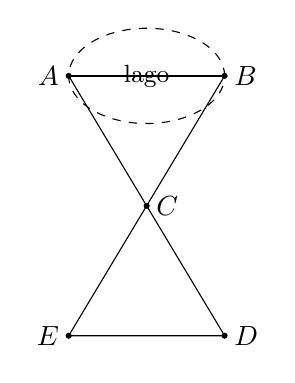
\begin{tikzpicture}[scale=0.55]
  \draw[dashed] (0,0) ellipse (1.8 and 1.1);
  \node at (0,0) {\small lago};
  \coordinate (A) at (-1.8,0); \coordinate (B) at (1.8,0);
  \coordinate (C) at (0,-3);
  \coordinate (D) at (1.8,-6); \coordinate (E) at (-1.8,-6);
  \draw (A) -- (D) (B) -- (E) (D) -- (E);
  \draw[thick] (A) -- (B);
  \foreach \p/\pos in {A/left, B/right, C/right, D/right, E/left}
    \fill (\p) circle (2pt) node[\pos] {$\p$};
\end{tikzpicture}
\end{center}
\end{ejemplo}

\begin{aplicacion}[El triángulo rígido]
Por el criterio LLL, si se fijan los tres lados de un triángulo, su forma queda
fija: un triángulo de listones no se deforma, mientras que un cuadrado sí. Por eso
las cerchas de los techos, las torres de energía y muchos puentes están hechos de
triángulos.
\end{aplicacion}

\begin{preguntas}
% Ejercicio: triangulos-8-008
\pregunta Indica si la afirmación es verdadera o falsa y argumenta tu respuesta (las
figuras están en un plano): «Si la mediana de la base de un triángulo es
perpendicular a la base, entonces el triángulo es isósceles». (Pista: la mediana
divide al triángulo en dos triángulos; ¿son congruentes? ¿Por qué criterio?)
\renglones{4}
% Ejercicio: triangulos-8-011
\pregunta Indica si la afirmación es verdadera o falsa y argumenta tu respuesta (las
figuras están en un plano): «Si la mediatriz de la base de un triángulo coincide con
la bisectriz del ángulo del vértice opuesto a la base, entonces el triángulo es
isósceles».
\renglones{4}
% Ejercicio: triangulos-8-012
\pregunta Indica si la afirmación es verdadera o falsa y argumenta tu respuesta (las
figuras están en un plano): «Una perpendicular a la bisectriz de un ángulo forma un
triángulo isósceles con los lados del ángulo». (Pista: ¿qué criterio de congruencia
puedes usar en los dos triángulos que forma la bisectriz?)
\renglones{4}
\end{preguntas}

\begin{resumen}
\begin{itemize}
  \item Congruentes: misma forma y mismo tamaño (semejantes con $k = 1$).
  \item Criterios: LLL, LAL y ALA. AAA y LLA \emph{no} son criterios de congruencia.
  \item Con triángulos congruentes se miden longitudes inaccesibles copiándolas en un lugar accesible.
\end{itemize}
\end{resumen}

% ---------------------------------------------------------------------
\tema{Teorema de Thales}\label{tema:thales}

\begin{hilo}
Mediodía del solsticio. En Siena, el Sol cae vertical; en Alejandría, el gnomon
proyecta una sombra corta. Eratóstenes imagina los rayos del Sol como rectas
paralelas que atraviesan la Tierra y se pregunta: ¿qué ángulo forman los dos
gnomones, prolongados, en el centro del planeta?
\end{hilo}

\begin{teorema}[Teorema de Thales]
Si tres o más rectas paralelas cortan a dos rectas secantes, los segmentos que
determinan en una secante son proporcionales a los segmentos correspondientes en la
otra: $\dfrac{AB}{BC} = \dfrac{A'B'}{B'C'}$.
\end{teorema}

\begin{center}
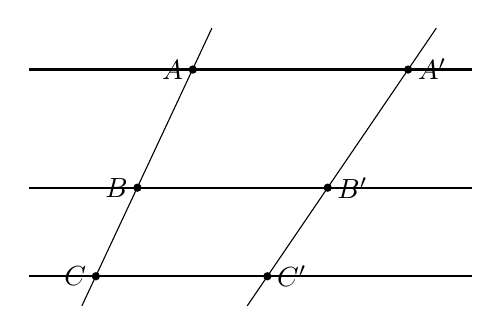
\begin{tikzpicture}[scale=0.75]
  \foreach \y/\n in {0/C, 1.5/B, 3.5/A} \draw[thick] (-0.5,\y) -- (7,\y);
  \draw (0.4,-0.5) -- (2.6,4.2);
  \draw (3.2,-0.5) -- (6.4,4.2);
  \foreach \x/\y/\n in {0.636/0/C, 1.340/1.5/B, 2.277/3.5/A}
    \fill (\x,\y) circle (2pt) node[left] {$\n$};
  \foreach \x/\y/\n in {3.540/0/C', 4.562/1.5/B', 5.923/3.5/A'}
    \fill (\x,\y) circle (2pt) node[right] {$\n$};
\end{tikzpicture}

{\small Tres paralelas (horizontales) cortan dos secantes.}
\end{center}

Una consecuencia muy útil: si en el triángulo $ABC$ se traza $DE$ paralela a $BC$
($D$ en $AB$, $E$ en $AC$), entonces $\frac{AD}{DB} = \frac{AE}{EC}$, y el triángulo
$ADE$ es semejante al $ABC$ (criterio AA, por los ángulos correspondientes entre
paralelas). Recíprocamente, si $\frac{AD}{DB} = \frac{AE}{EC}$, entonces $DE \parallel BC$.

\begin{ejemplo}[El ángulo de Eratóstenes]
El rayo que llega a Alejandría es paralelo al que llega a Siena, y este pasa por el
centro $O$ de la Tierra. El gnomon de Alejandría, prolongado, también pasa por $O$.
Esa prolongación es una secante de las dos paralelas, así que el ángulo de la sombra
en Alejandría y el ángulo en $O$ son \emph{alternos internos}: son iguales. Si el
ángulo mide $\frac{1}{50}$ de circunferencia, el arco Siena--Alejandría es
$\frac{1}{50}$ de la circunferencia de la Tierra.
\begin{center}
\begin{tikzpicture}[scale=1]
  \draw (0,0) circle (2);
  \fill (0,0) circle (1.5pt) node[below] {$O$};
  % gnomones prolongados hasta el centro
  \draw (0,0) -- (90:2.6);
  \draw (0,0) -- (60:2.6);
  \node[left, font=\small] at (90:2.35) {Siena};
  \node[right, font=\small] at (60:2.45) {Alejandría};
  % rayos del Sol, verticales y paralelos
  \draw[->, dashed] (-0.9,4.4) -- (-0.9,2.0);
  \draw[->, dashed] (0,4.4) -- (0,2.65);
  \draw[->, dashed] ($(60:2.6)+(0,1.8)$) -- (60:2.6);
  \node[align=left, font=\small] at (3.3,4.0) {rayos del Sol\\(paralelos)};
  % el ángulo en el centro y el de la sombra (alternos internos)
  \draw (90:0.7) arc (90:60:0.7);
  \node[font=\small] at (75:1.0) {$\alpha$};
  \draw ($(60:2.6)+(0,0.55)$) arc (90:60:0.55);
  \node[font=\small] at ($(60:2.6)+(75:0.85)$) {$\alpha$};
\end{tikzpicture}

{\small El ángulo $\alpha$ de la sombra en Alejandría es igual al ángulo en el centro $O$.}
\end{center}
\end{ejemplo}

\begin{aplicacion}[Alturas con sombras]
A una misma hora, los rayos del Sol llegan paralelos a todo el colegio. Un palo
vertical y su sombra forman un triángulo rectángulo semejante al que forman un
edificio y la suya. Midiendo tres longitudes en el suelo se calcula la cuarta: la
altura del edificio. Así se miden árboles, postes y torres sin subirse a ellos.
\end{aplicacion}

\begin{preguntas}
% Ejercicio: triangulos-8-006
\pregunta Indica si la afirmación es verdadera o falsa y argumenta tu respuesta (las
figuras están en un plano): «Si se dibuja una recta paralela a la base de un
triángulo isósceles que pase por el vértice opuesto, esta formará dos ángulos de la
misma medida con los lados del triángulo». (Es el mismo razonamiento de ángulos
entre paralelas que usó Eratóstenes.)
\renglones{4}
% Ejercicio: semejanza-escala-5-007
\pregunta Tania quiere saber la altura del asta de la bandera que está frente a su
escuela. A la misma hora, la sombra de una regla de 1 m mide 2 m y la sombra del
asta mide \num{20,2} m. ¿Cuál es la altura del asta? Explica por qué los dos
triángulos son semejantes.
\espacio{3cm}
\end{preguntas}

\begin{resumen}
\begin{itemize}
  \item Paralelas cortadas por secantes determinan segmentos proporcionales.
  \item Una paralela a un lado de un triángulo forma un triángulo semejante al original.
  \item Con rayos paralelos (el Sol), una sombra permite medir alturas y hasta el tamaño de la Tierra.
\end{itemize}
\end{resumen}

% ---------------------------------------------------------------------
\tema{Teorema de Pitágoras}\label{tema:pitagoras}

\begin{hilo}
Con la circunferencia de la Tierra, Eratóstenes podía calcular su radio y, con él,
muchas otras distancias. Casi todas esas cuentas pasan por triángulos rectángulos:
el teorema que los gobierna es el de Pitágoras.
\end{hilo}

\begin{teorema}[Teorema de Pitágoras]
En todo triángulo rectángulo, el cuadrado de la hipotenusa es igual a la suma de
los cuadrados de los catetos: $c^2 = a^2 + b^2$. \textbf{Recíproco:} si los lados de
un triángulo cumplen $c^2 = a^2 + b^2$, el triángulo es rectángulo.
\end{teorema}

\emph{Demostración por áreas.} Un cuadrado de lado $a + b$ se puede llenar de dos
maneras: con cuatro copias del triángulo rectángulo alrededor de un cuadrado
inclinado de lado $c$, o con un cuadrado de lado $a$, uno de lado $b$ y dos
rectángulos de $a \times b$. Igualando las áreas,
$c^2 + 4 \cdot \frac{ab}{2} = a^2 + b^2 + 2ab$, y queda $c^2 = a^2 + b^2$. La
prueba de Garfield usa la mitad de esta figura: un trapecio formado por dos copias
del triángulo y un triángulo rectángulo isósceles de catetos $c$.

\begin{center}
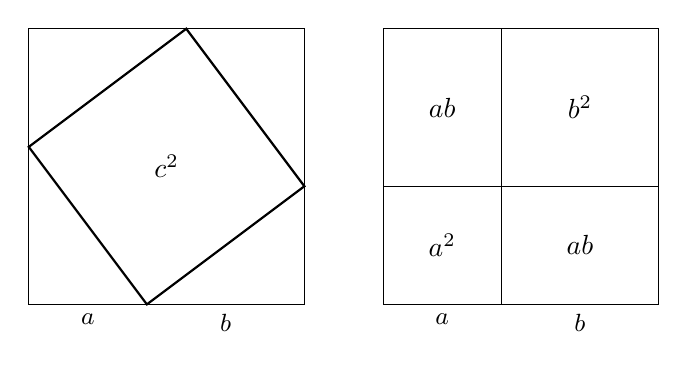
\begin{tikzpicture}[scale=0.5]
  \draw (0,0) rectangle (7,7);
  \draw[thick] (3,0) -- (7,3) -- (4,7) -- (0,4) -- cycle;
  \node[below] at (1.5,0) {\small $a$}; \node[below] at (5,0) {\small $b$};
  \node at (3.5,3.5) {$c^2$};
  \begin{scope}[xshift=9cm]
    \draw (0,0) rectangle (7,7);
    \draw (3,0) -- (3,7) (0,3) -- (7,3);
    \node at (1.5,1.5) {$a^2$}; \node at (5,5) {$b^2$};
    \node at (5,1.5) {$ab$}; \node at (1.5,5) {$ab$};
    \node[below] at (1.5,0) {\small $a$}; \node[below] at (5,0) {\small $b$};
  \end{scope}
\end{tikzpicture}
\end{center}

% Ejemplo del recurso: módulo de Geometría, Tema 3, Ejemplo 6, con el dato del enunciado (1,25 m): sqrt(3,5² + 1,25²) = sqrt(13,8125) ≈ 3,72
\begin{ejemplo}[Un cable tensor]
A un poste de energía se le pone un cable tensor desde una altura de
$\num{3,5}$~m hasta un punto del suelo a $\num{1,25}$~m de la base. El poste, el
suelo y el cable forman un triángulo rectángulo, y el cable es la hipotenusa:
$c = \sqrt{\num{3,5}^2 + \num{1,25}^2} = \sqrt{\num{13,8125}} \approx \num{3,72}$~m
(sin contar lo que se necesita para amarrarlo).
\end{ejemplo}

\begin{aplicacion}[La escuadra de los maestros de obra]
Para comprobar que la esquina de un muro o de una cancha es recta, los maestros de
obra marcan $60$~cm en un lado y $80$~cm en el otro: si la distancia entre las marcas
es exactamente $100$~cm, el ángulo es recto, por el recíproco del teorema
($60^2 + 80^2 = 100^2$). No necesitan transportador.
\end{aplicacion}

\begin{preguntas}
% Ejercicio: pitagoras-9-001
\pregunta ¿Qué longitudes irracionales puedes obtener al dibujar triángulos
rectángulos que tengan dos lados de $9$~cm y $7$~cm?
\espacio{3cm}
% Ejercicio: pitagoras-9-005
\pregunta ¿Cuánto mide la diagonal de un rectángulo de base $7$~cm y altura $6$~cm?
\espacio{2cm}
% Ejercicio: pitagoras-9-006
\pregunta ¿Cuánto mide la diagonal de un rectángulo de base $10$~cm y área $50$~cm$^2$?
\espacio{2.5cm}
\end{preguntas}

\begin{resumen}
\begin{itemize}
  \item En un triángulo rectángulo, $c^2 = a^2 + b^2$; la hipotenusa es el lado mayor.
  \item El recíproco sirve para comprobar ángulos rectos midiendo solo longitudes.
  \item Muchas distancias que no se pueden medir directamente son hipotenusas o catetos de un triángulo rectángulo.
\end{itemize}
\end{resumen}

% ---------------------------------------------------------------------
\tema{Estrategias de medición}\label{tema:medicion}

\begin{hilo}
Eratóstenes obtuvo 250\,000 estadios. ¿Acertó? Depende de cuánto medía su estadio,
de qué tan bien se midió la distancia entre las ciudades y de qué tan preciso fue su
ángulo. Toda medición tiene un margen de error: medir bien es también saber cuánto
nos podemos equivocar.
\end{hilo}

Una \textbf{estrategia de medición indirecta} tiene tres partes: una figura
geométrica que relaciona lo que se quiere medir con lo que sí se puede medir
(triángulos semejantes, congruentes o rectángulos); un instrumento para tomar esas
medidas; y una justificación con un teorema. Para que el resultado sea confiable:
\begin{itemize}
  \item se escoge el instrumento adecuado (una cinta métrica y no los pasos; una
        plomada o un nivel para asegurar la vertical);
  \item se mide varias veces y se usa el \textbf{promedio};
  \item se reporta el resultado con un \textbf{margen} (por ejemplo, $\num{9,2} \pm
        \num{0,2}$~m) y con las cifras que las medidas permiten, no más;
  \item se comprueba, si es posible, con otro método.
\end{itemize}

% Ejemplo del DBA 5 de grado 9 (MEN): escuadra isósceles de Camila; H = d por ser 45°
\begin{ejemplo}[La escuadra de Camila (ejemplo del DBA)]
Camila pega un pitillo a la hipotenusa de una escuadra isósceles y cuelga una
plomada para que un cateto quede vertical. Así, por el pitillo mira siempre a
$45^\circ$ sobre la horizontal. Se aleja o se acerca del árbol hasta ver el ave por el
pitillo. En ese momento, el triángulo formado por la visual, la horizontal de sus
ojos y el tronco es rectángulo e isósceles: la altura $H$ del ave sobre sus ojos es
igual a su distancia $d$ al árbol. La altura del ave es $h + H$, donde $h$ es la
altura de los ojos de Camila.
\begin{center}
\begin{tikzpicture}[scale=0.5]
  \draw (-1,0) -- (8,0);
  \draw[thick] (6,0) -- (6,8.3);
  \fill (6,7.6) circle (4pt) node[right=2pt] {\small ave};
  \draw (0,0) -- (0,1.6);
  \fill (0,1.6) circle (2pt);
  \draw[dashed] (0,1.6) -- (6,1.6);
  \draw[dashed] (0,1.6) -- (6,7.6);
  \draw (1.2,1.6) arc (0:45:1.2); \node[font=\scriptsize] at (2.1,2.05) {$45^\circ$};
  \draw[<->] (0,-0.7) -- node[below] {\small $d$} (6,-0.7);
  \draw[<->] (-0.6,0) -- node[left] {\small $h$} (-0.6,1.6);
  \draw[<->] (6.9,1.6) -- node[right] {\small $H = d$} (6.9,7.6);
\end{tikzpicture}
\end{center}
\end{ejemplo}

\begin{aplicacion}[La topografía]
Los topógrafos que trazan una carretera o delimitan un lote no miden todo con
cinta: miden algunos ángulos y algunas distancias, y calculan el resto con
triángulos. Sus instrumentos (teodolitos y estaciones totales) miden ángulos con
mucha más precisión que un transportador escolar, porque un error pequeño en un
ángulo se convierte en un error grande en una distancia lejana.
\end{aplicacion}

\begin{preguntas}
% Ejercicio: medicion-indirecta-9-006
\pregunta Camila mira un ave por un pitillo pegado a la hipotenusa de una escuadra
isósceles ($45^\circ$), con una plomada que mantiene un cateto vertical. Se acerca al
árbol hasta ver el ave por el pitillo; en ese punto mide la distancia al árbol,
$d = \num{8,4}$~m. Sus ojos están a $h = \num{1,55}$~m del suelo. ¿A qué altura está
el ave? Justifica.
\espacio{3cm}
% Ejercicio: medicion-indirecta-9-008
\pregunta Para medir el asta de la bandera del colegio, un palo de $\num{1,20}$~m da
una sombra de $\num{0,80}$~m. Cuatro estudiantes miden la sombra del asta y obtienen
$\num{6,10}$, $\num{6,25}$, $\num{6,05}$ y $\num{6,20}$~m.
\begin{opciones}
  \item Calcula la altura con el promedio.
  \item ¿Entre qué valores está la altura según la medida más pequeña y la más grande?
  \item ¿Cómo reportarías el resultado?
\end{opciones}
\espacio{3.5cm}
\end{preguntas}

\begin{resumen}
\begin{itemize}
  \item Una medición indirecta combina una figura, un instrumento y un teorema que la justifica.
  \item Medir varias veces, promediar y dar un margen hace confiable el resultado.
  \item Los errores de ángulo pesan mucho en las distancias grandes: por eso la precisión del instrumento importa.
\end{itemize}
\end{resumen}

% ---------------------------------------------------------------------
% 5. Prepárate para Saber 11
% ---------------------------------------------------------------------
\seccion{Prepárate para Saber 11}

\begin{instrucciones}
Preguntas de selección múltiple con única respuesta, como las de la prueba Saber 11.
Las tres son del cuadernillo oficial de preguntas del Icfes~\cite{icfes2026}
(preguntas 15, 14 y 41) y se reproducen sin cambios.
\end{instrucciones}

\begin{preguntas}
% Ejercicio: icfes-cuadernillo-2026-015
\Needspace{22\baselineskip}
\pregunta Las sombras proyectadas por dos postes paralelos de 10 metros y 5 metros
se muestran en la figura.

\begin{center}
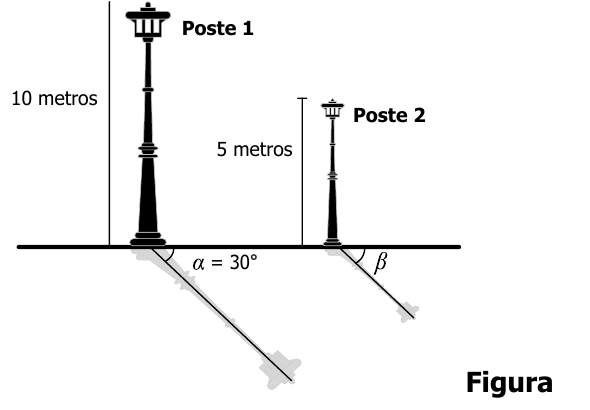
\includegraphics[width=0.55\linewidth]{figuras/icfes-2026-p15.png}
\end{center}

El ángulo entre la acera horizontal y la sombra del poste 1 es $\alpha = 30^\circ$.
De acuerdo con esto, se puede afirmar que el ángulo entre la acera horizontal y la
sombra del poste 2 es
\begin{opciones*}(4)
  \item $\beta = 5^\circ$.
  \item $\beta = 15^\circ$.
  \item $\beta = 30^\circ$.
  \item $\beta = 60^\circ$.
\end{opciones*}
% Ejercicio: icfes-cuadernillo-2026-014
\pregunta Si en un rectángulo se aumenta la longitud de uno de sus lados en
100~\%, ¿Qué se puede concluir de su área?
\begin{opciones*}(2)
  \item Aumenta en un 50~\%.
  \item Se duplica.
  \item No cambia.
  \item Aumenta en 100 unidades.
\end{opciones*}
% Ejercicio: icfes-cuadernillo-2026-041
\pregunta Un terreno con forma triangular se debe encerrar, cumpliendo con los
siguientes requerimientos:
\textbf{Requerimiento 1.} Uno de sus ángulos interiores debe ser de 90°.
\textbf{Requerimiento 2.} Dos lados deben medir 7 metros y el otro debe medir 18
metros. \textbf{Requerimiento 3.} Uno de sus ángulos interiores debe ser menor que
45°. \textbf{Requerimiento 4.} La suma de sus ángulos interiores debe ser de 180°.
¿Cuál de los requerimientos es \textbf{imposible} de cumplir?
\begin{opciones*}(4)
  \item Requerimiento 1.
  \item Requerimiento 2.
  \item Requerimiento 3.
  \item Requerimiento 4.
\end{opciones*}
\end{preguntas}

% ---------------------------------------------------------------------
% 6. Cierre del hilo conductor
% ---------------------------------------------------------------------
\seccion{Cierre: la sombra que midió el mundo}

Eratóstenes nunca salió de Egipto para medir la Tierra. Le bastaron una sombra,
rayos paralelos, un ángulo y una proporción: la geometría de este trimestre. Su
método era tan bueno que hoy lo repiten colegios de todo el mundo, y su única
debilidad ---la longitud del estadio--- nos enseñó que una medida vale tanto como
la precisión con que se tomó. Henrietta Leavitt llevó la misma idea hasta otras
galaxias. En el segundo trimestre pasaremos de las longitudes a los volúmenes:
cilindros, conos y esferas, y la capacidad de los objetos que usamos cada día.

% ---------------------------------------------------------------------
% 7. Evaluación (secciones institucionales)
% ---------------------------------------------------------------------
\matrizevaluacion
  {Explica los criterios de semejanza y congruencia y los teoremas de Thales y
   Pitágoras, y reconoce cuándo se aplica cada uno.}
  {Propone y justifica estrategias de medición indirecta, calcula longitudes con
   triángulos semejantes o rectángulos y estima el margen de error de sus medidas.}
  {Argumenta sus procedimientos y revisa los de otros con criterios geométricos, sin
   conformarse con «se ve que sí».}
  {Colabora en las mediciones de grupo, respeta los datos de sus compañeros y valora
   el aporte de mujeres y hombres de distintas épocas a la ciencia.}

\autoevaluacion

\seguimientodocente

% ---------------------------------------------------------------------
% 8. Referencias
% ---------------------------------------------------------------------
\begin{referencias}
% verificado: https://bmcr.brynmawr.edu/2004/2004.08.06/ — UC Press 2004 (Hellenistic Culture and Society 42); cap. 7: la determinación de Eratóstenes
\bibitem{cleomedes} Bowen, A. C. y Todd, R. B. (2004). \emph{Cleomedes' Lectures on
  Astronomy: A Translation of The Heavens}. Berkeley: University of California Press.
% verificado: https://portalegalileo.museogalileo.it/egjr.asp?c=36261 — Roma: Giacomo Mascardi, 1623
\bibitem{galileo1623} Galilei, G. (1623). \emph{Il Saggiatore}. Roma: Giacomo Mascardi.
% verificado: https://www.scientificamerican.com/blog/observations/presidential-pythagorean-proof/ — New-England Journal of Education, 1876; Garfield, congresista de Ohio
\bibitem{garfield} Garfield, J. A. (1876). [Demostración del teorema de Pitágoras].
  \emph{New-England Journal of Education}, 3(14), 161.
% verificado: recursos/matematicas/icfes/09-Marzo_Cuadernillo-de-Preguntas-Matematicas-Saber-11-2026.pdf (archivo local) — Icfes, marzo de 2026
\bibitem{icfes2026} Icfes (2026). \emph{Cuadernillo de preguntas Saber 11.º: prueba de
  Matemáticas}. Bogotá: Instituto Colombiano para la Evaluación de la Educación.
% verificado: https://ui.adsabs.harvard.edu/abs/1912HarCi.173....1L/abstract — Harvard College Observatory Circular 173 (1912), pp. 1–3
\bibitem{leavitt} Leavitt, H. S. y Pickering, E. C. (1912). Periods of 25 variable
  stars in the Small Magellanic Cloud. \emph{Harvard College Observatory Circular},
  173, 1--3.
% verificado: https://mathshistory.st-andrews.ac.uk/Biographies/Eratosthenes/ — 276–194 a. C.; tercer bibliotecario; «Beta»; 250 000 estadios; estadio de 157,2 o 166,7 m
\bibitem{mactutoreratostenes} O'Connor, J. J. y Robertson, E. F. (1999).
  \emph{Eratosthenes of Cyrene}. MacTutor History of Mathematics, University of St Andrews.
% verificado: https://gblumen.mineducacion.gov.co/cgi-bin/koha/opac-detail.pl?biblionumber=4785 — MEN 2016
\bibitem{mendba} Ministerio de Educación Nacional (2016). \emph{Derechos Básicos de
  Aprendizaje V.2: Matemáticas}. Bogotá: MEN.
% verificado: recursos/matematicas/Guías pedagógicas Matemáticas/Modulo_Matematicas_Geometria.docx (archivo local) — autora y título de la portada
\bibitem{quintero} Quintero Palomino, A. (s.\,f.). \emph{Conceptos de la geometría plana y
  la representación y caracterización de ángulos y figuras geométricas} (Guía de apoyo
  educativo en el área de las matemáticas).
\end{referencias}

\end{document}
